% !TeX program = pdflatex
% !TeX root = DiracTrace.tex

\documentclass[../FeynCalcManual.tex]{subfiles}
\begin{document}
\begin{Shaded}
\begin{Highlighting}[]
 
\end{Highlighting}
\end{Shaded}

\hypertarget{diractrace}{
\section{DiracTrace}\label{diractrace}\index{DiracTrace}}

\texttt{DiracTrace[\allowbreak{}exp]} is the head of Dirac traces. By
default the trace is not evaluated. The evaluation occurs only when the
option \texttt{DiracTraceEvaluate} is set to \texttt{True}. It is
recommended to use \texttt{DiracSimplify}, which will automatically
evaluate all Dirac traces in the input expression.

\subsection{See also}

\hyperlink{toc}{Overview}, \hyperlink{contract}{Contract},
\hyperlink{diracequation}{DiracEquation},
\hyperlink{diracgamma}{DiracGamma},
\hyperlink{diracgammaexpand}{DiracGammaExpand},
\hyperlink{diractrick}{DiracTrick},
\hyperlink{fcgetdiracgammascheme}{FCGetDiracGammaScheme},
\hyperlink{fcsetdiracgammascheme}{FCSetDiracGammaScheme}.

\subsection{Examples}

There is no automatic evaluation of Dirac traces

\begin{Shaded}
\begin{Highlighting}[]
\NormalTok{DiracTrace}\OperatorTok{[}\NormalTok{GA}\OperatorTok{[}\SpecialCharTok{\textbackslash{}}\OperatorTok{[}\NormalTok{Mu}\OperatorTok{],} \SpecialCharTok{\textbackslash{}}\OperatorTok{[}\NormalTok{Nu}\OperatorTok{]]]}
\end{Highlighting}
\end{Shaded}

\begin{dmath*}\breakingcomma
\text{tr}\left(\bar{\gamma }^{\mu }.\bar{\gamma }^{\nu }\right)
\end{dmath*}

\begin{Shaded}
\begin{Highlighting}[]
\NormalTok{DiracTrace}\OperatorTok{[}\NormalTok{GA}\OperatorTok{[}\SpecialCharTok{\textbackslash{}}\OperatorTok{[}\NormalTok{Mu}\OperatorTok{],} \SpecialCharTok{\textbackslash{}}\OperatorTok{[}\NormalTok{Nu}\OperatorTok{],} \SpecialCharTok{\textbackslash{}}\OperatorTok{[}\NormalTok{Rho}\OperatorTok{],} \SpecialCharTok{\textbackslash{}}\OperatorTok{[}\NormalTok{Sigma}\OperatorTok{]]]}
\end{Highlighting}
\end{Shaded}

\begin{dmath*}\breakingcomma
\text{tr}\left(\bar{\gamma }^{\mu }.\bar{\gamma }^{\nu }.\bar{\gamma }^{\rho }.\bar{\gamma }^{\sigma }\right)
\end{dmath*}

You can either set the option \texttt{DiracTraceEvaluate} to
\texttt{True} or use \texttt{DiracSimplify}.

\begin{Shaded}
\begin{Highlighting}[]
\NormalTok{DiracTrace}\OperatorTok{[}\NormalTok{GA}\OperatorTok{[}\SpecialCharTok{\textbackslash{}}\OperatorTok{[}\NormalTok{Mu}\OperatorTok{],} \SpecialCharTok{\textbackslash{}}\OperatorTok{[}\NormalTok{Nu}\OperatorTok{],} \SpecialCharTok{\textbackslash{}}\OperatorTok{[}\NormalTok{Rho}\OperatorTok{],} \SpecialCharTok{\textbackslash{}}\OperatorTok{[}\NormalTok{Sigma}\OperatorTok{]],}\NormalTok{ DiracTraceEvaluate }\OtherTok{{-}\textgreater{}} \ConstantTok{True}\OperatorTok{]}
\end{Highlighting}
\end{Shaded}

\begin{dmath*}\breakingcomma
4 \left(\bar{g}^{\mu \sigma } \bar{g}^{\nu \rho }-\bar{g}^{\mu \rho } \bar{g}^{\nu \sigma }+\bar{g}^{\mu \nu } \bar{g}^{\rho \sigma }\right)
\end{dmath*}

\begin{Shaded}
\begin{Highlighting}[]
\NormalTok{DiracSimplify}\OperatorTok{[}\NormalTok{DiracTrace}\OperatorTok{[}\NormalTok{GA}\OperatorTok{[}\SpecialCharTok{\textbackslash{}}\OperatorTok{[}\NormalTok{Mu}\OperatorTok{],} \SpecialCharTok{\textbackslash{}}\OperatorTok{[}\NormalTok{Nu}\OperatorTok{],} \SpecialCharTok{\textbackslash{}}\OperatorTok{[}\NormalTok{Rho}\OperatorTok{],} \SpecialCharTok{\textbackslash{}}\OperatorTok{[}\NormalTok{Sigma}\OperatorTok{]]]]}
\end{Highlighting}
\end{Shaded}

\begin{dmath*}\breakingcomma
4 \bar{g}^{\mu \sigma } \bar{g}^{\nu \rho }-4 \bar{g}^{\mu \rho } \bar{g}^{\nu \sigma }+4 \bar{g}^{\mu \nu } \bar{g}^{\rho \sigma }
\end{dmath*}

\begin{Shaded}
\begin{Highlighting}[]
\NormalTok{DiracTrace}\OperatorTok{[}\NormalTok{GS}\OperatorTok{[}\FunctionTok{p}\OperatorTok{,} \FunctionTok{q}\OperatorTok{,} \FunctionTok{r}\OperatorTok{,} \FunctionTok{s}\OperatorTok{]]} 
 
\NormalTok{DiracSimplify}\OperatorTok{[}\SpecialCharTok{\%}\OperatorTok{]}
\end{Highlighting}
\end{Shaded}

\begin{dmath*}\breakingcomma
\text{tr}\left(\left(\bar{\gamma }\cdot \overline{p}\right).\left(\bar{\gamma }\cdot \overline{q}\right).\left(\bar{\gamma }\cdot \overline{r}\right).\left(\bar{\gamma }\cdot \overline{s}\right)\right)
\end{dmath*}

\begin{dmath*}\breakingcomma
4 \left(\overline{p}\cdot \overline{s}\right) \left(\overline{q}\cdot \overline{r}\right)-4 \left(\overline{p}\cdot \overline{r}\right) \left(\overline{q}\cdot \overline{s}\right)+4 \left(\overline{p}\cdot \overline{q}\right) \left(\overline{r}\cdot \overline{s}\right)
\end{dmath*}

The old methods of evaluating traces by replacing \texttt{DiracTrace}
with \texttt{Tr} or \texttt{TR} are deprecated and should not be used
anymore. In particular, they are slower are less efficient than using
\texttt{DiracSimplify}.

Traces involving \(\gamma^5\) or chirality projectors in \(4\)
dimensions are also possible

\begin{Shaded}
\begin{Highlighting}[]
\NormalTok{DiracTrace}\OperatorTok{[}\NormalTok{GA}\OperatorTok{[}\SpecialCharTok{\textbackslash{}}\OperatorTok{[}\NormalTok{Mu}\OperatorTok{],} \SpecialCharTok{\textbackslash{}}\OperatorTok{[}\NormalTok{Nu}\OperatorTok{],} \SpecialCharTok{\textbackslash{}}\OperatorTok{[}\NormalTok{Rho}\OperatorTok{],} \SpecialCharTok{\textbackslash{}}\OperatorTok{[}\NormalTok{Sigma}\OperatorTok{],} \DecValTok{5}\OperatorTok{]]} 
 
\NormalTok{DiracSimplify}\OperatorTok{[}\SpecialCharTok{\%}\OperatorTok{]}
\end{Highlighting}
\end{Shaded}

\begin{dmath*}\breakingcomma
\text{tr}\left(\bar{\gamma }^{\mu }.\bar{\gamma }^{\nu }.\bar{\gamma }^{\rho }.\bar{\gamma }^{\sigma }.\bar{\gamma }^5\right)
\end{dmath*}

\begin{dmath*}\breakingcomma
-4 i \bar{\epsilon }^{\mu \nu \rho \sigma }
\end{dmath*}

\begin{Shaded}
\begin{Highlighting}[]
\NormalTok{DiracTrace}\OperatorTok{[}\NormalTok{GA}\OperatorTok{[}\SpecialCharTok{\textbackslash{}}\OperatorTok{[}\NormalTok{Mu}\OperatorTok{],} \SpecialCharTok{\textbackslash{}}\OperatorTok{[}\NormalTok{Nu}\OperatorTok{],} \SpecialCharTok{\textbackslash{}}\OperatorTok{[}\NormalTok{Rho}\OperatorTok{],} \SpecialCharTok{\textbackslash{}}\OperatorTok{[}\NormalTok{Sigma}\OperatorTok{],} \SpecialCharTok{\textbackslash{}}\OperatorTok{[}\NormalTok{Delta}\OperatorTok{],} \SpecialCharTok{\textbackslash{}}\OperatorTok{[}\NormalTok{Tau}\OperatorTok{],} \DecValTok{5}\OperatorTok{]]} 
 
\NormalTok{DiracSimplify}\OperatorTok{[}\SpecialCharTok{\%}\OperatorTok{]}
\end{Highlighting}
\end{Shaded}

\begin{dmath*}\breakingcomma
\text{tr}\left(\bar{\gamma }^{\mu }.\bar{\gamma }^{\nu }.\bar{\gamma }^{\rho }.\bar{\gamma }^{\sigma }.\bar{\gamma }^{\delta }.\bar{\gamma }^{\tau }.\bar{\gamma }^5\right)
\end{dmath*}

\begin{dmath*}\breakingcomma
-4 i \bar{g}^{\delta \mu } \bar{\epsilon }^{\nu \rho \sigma \tau }-4 i \bar{g}^{\delta \tau } \bar{\epsilon }^{\mu \nu \rho \sigma }-4 i \bar{g}^{\mu \tau } \bar{\epsilon }^{\delta \nu \rho \sigma }-4 i \bar{g}^{\nu \rho } \bar{\epsilon }^{\delta \mu \sigma \tau }+4 i \bar{g}^{\nu \sigma } \bar{\epsilon }^{\delta \mu \rho \tau }-4 i \bar{g}^{\rho \sigma } \bar{\epsilon }^{\delta \mu \nu \tau }
\end{dmath*}

\begin{Shaded}
\begin{Highlighting}[]
\NormalTok{DiracTrace}\OperatorTok{[}\NormalTok{GA}\OperatorTok{[}\SpecialCharTok{\textbackslash{}}\OperatorTok{[}\NormalTok{Mu}\OperatorTok{],} \SpecialCharTok{\textbackslash{}}\OperatorTok{[}\NormalTok{Nu}\OperatorTok{],} \SpecialCharTok{\textbackslash{}}\OperatorTok{[}\NormalTok{Rho}\OperatorTok{],} \SpecialCharTok{\textbackslash{}}\OperatorTok{[}\NormalTok{Sigma}\OperatorTok{],} \SpecialCharTok{\textbackslash{}}\OperatorTok{[}\NormalTok{Delta}\OperatorTok{],} \SpecialCharTok{\textbackslash{}}\OperatorTok{[}\NormalTok{Tau}\OperatorTok{],} \DecValTok{6}\OperatorTok{]]} 
 
\NormalTok{DiracSimplify}\OperatorTok{[}\SpecialCharTok{\%}\OperatorTok{]}
\end{Highlighting}
\end{Shaded}

\begin{dmath*}\breakingcomma
\text{tr}\left(\bar{\gamma }^{\mu }.\bar{\gamma }^{\nu }.\bar{\gamma }^{\rho }.\bar{\gamma }^{\sigma }.\bar{\gamma }^{\delta }.\bar{\gamma }^{\tau }.\bar{\gamma }^6\right)
\end{dmath*}

\begin{dmath*}\breakingcomma
-2 \bar{g}^{\delta \mu } \bar{g}^{\nu \tau } \bar{g}^{\rho \sigma }+2 \bar{g}^{\delta \mu } \bar{g}^{\nu \sigma } \bar{g}^{\rho \tau }-2 \bar{g}^{\delta \mu } \bar{g}^{\nu \rho } \bar{g}^{\sigma \tau }+2 \bar{g}^{\delta \tau } \bar{g}^{\mu \sigma } \bar{g}^{\nu \rho }+2 \bar{g}^{\delta \sigma } \bar{g}^{\mu \tau } \bar{g}^{\nu \rho }-2 \bar{g}^{\delta \tau } \bar{g}^{\mu \rho } \bar{g}^{\nu \sigma }-2 \bar{g}^{\delta \rho } \bar{g}^{\mu \tau } \bar{g}^{\nu \sigma }-2 \bar{g}^{\delta \sigma } \bar{g}^{\mu \rho } \bar{g}^{\nu \tau }+2 \bar{g}^{\delta \rho } \bar{g}^{\mu \sigma } \bar{g}^{\nu \tau }+2 \bar{g}^{\delta \tau } \bar{g}^{\mu \nu } \bar{g}^{\rho \sigma }+2 \bar{g}^{\delta \nu } \bar{g}^{\mu \tau } \bar{g}^{\rho \sigma }+2 \bar{g}^{\delta \sigma } \bar{g}^{\mu \nu } \bar{g}^{\rho \tau }-2 \bar{g}^{\delta \nu } \bar{g}^{\mu \sigma } \bar{g}^{\rho \tau }-2 \bar{g}^{\delta \rho } \bar{g}^{\mu \nu } \bar{g}^{\sigma \tau }+2 \bar{g}^{\delta \nu } \bar{g}^{\mu \rho } \bar{g}^{\sigma \tau }-2 i \bar{g}^{\delta \mu } \bar{\epsilon }^{\nu \rho \sigma \tau }-2 i \bar{g}^{\delta \tau } \bar{\epsilon }^{\mu \nu \rho \sigma }-2 i \bar{g}^{\mu \tau } \bar{\epsilon }^{\delta \nu \rho \sigma }-2 i \bar{g}^{\nu \rho } \bar{\epsilon }^{\delta \mu \sigma \tau }+2 i \bar{g}^{\nu \sigma } \bar{\epsilon }^{\delta \mu \rho \tau }-2 i \bar{g}^{\rho \sigma } \bar{\epsilon }^{\delta \mu \nu \tau }
\end{dmath*}

\(D\)-dimensional traces that do not involve \(\gamma^5\) are
unambiguous.

\begin{Shaded}
\begin{Highlighting}[]
\NormalTok{DiracTrace}\OperatorTok{[}\NormalTok{(}\SpecialCharTok{{-}}\NormalTok{GSD}\OperatorTok{[}\FunctionTok{q}\OperatorTok{]} \SpecialCharTok{+}\NormalTok{ SMP}\OperatorTok{[}\StringTok{"m\_e"}\OperatorTok{]}\NormalTok{) . GAD}\OperatorTok{[}\SpecialCharTok{\textbackslash{}}\OperatorTok{[}\NormalTok{Nu}\OperatorTok{]]}\NormalTok{ . (GSD}\OperatorTok{[}\FunctionTok{p} \SpecialCharTok{{-}} \FunctionTok{q}\OperatorTok{]} \SpecialCharTok{+}\NormalTok{ SMP}\OperatorTok{[}\StringTok{"m\_e"}\OperatorTok{]}\NormalTok{) . GAD}\OperatorTok{[}\SpecialCharTok{\textbackslash{}}\OperatorTok{[}\NormalTok{Mu}\OperatorTok{]]]} 
 
\NormalTok{DiracSimplify}\OperatorTok{[}\SpecialCharTok{\%}\OperatorTok{]}
\end{Highlighting}
\end{Shaded}

\begin{dmath*}\breakingcomma
\text{tr}\left(\left(m_e-\gamma \cdot q\right).\gamma ^{\nu }.\left(m_e+\gamma \cdot (p-q)\right).\gamma ^{\mu }\right)
\end{dmath*}

\begin{dmath*}\breakingcomma
4 m_e^2 g^{\mu \nu }+4 g^{\mu \nu } (p\cdot q)-4 q^2 g^{\mu \nu }-4 p^{\nu } q^{\mu }-4 p^{\mu } q^{\nu }+8 q^{\mu } q^{\nu }
\end{dmath*}

Traces that contain \(\gamma^5\) in \(D\) dimensions are
scheme-dependent. The default scheme used in FeynCalc is the naive
dimension regularization (NDR), where \(\gamma^5\) is assumed to
anticommute with all other Dirac matrices. However, chiral traces are
ambiguous in NDR, unless the trace contains an even number of
\(\gamma^5\). This is why FeynCalc will leave such traces unevaluated.

\begin{Shaded}
\begin{Highlighting}[]
\NormalTok{DiracTrace}\OperatorTok{[}\NormalTok{GAD}\OperatorTok{[}\SpecialCharTok{\textbackslash{}}\OperatorTok{[}\NormalTok{Mu}\OperatorTok{],} \SpecialCharTok{\textbackslash{}}\OperatorTok{[}\NormalTok{Nu}\OperatorTok{],} \SpecialCharTok{\textbackslash{}}\OperatorTok{[}\NormalTok{Rho}\OperatorTok{]]}\NormalTok{ . GA}\OperatorTok{[}\DecValTok{5}\OperatorTok{]}\NormalTok{ . GAD}\OperatorTok{[}\SpecialCharTok{\textbackslash{}}\OperatorTok{[}\NormalTok{Sigma}\OperatorTok{],} \SpecialCharTok{\textbackslash{}}\OperatorTok{[}\NormalTok{Delta}\OperatorTok{],} \SpecialCharTok{\textbackslash{}}\OperatorTok{[}\NormalTok{Tau}\OperatorTok{]]}\NormalTok{ . GA}\OperatorTok{[}\DecValTok{5}\OperatorTok{]]} 
 
\NormalTok{DiracSimplify}\OperatorTok{[}\SpecialCharTok{\%}\OperatorTok{]}
\end{Highlighting}
\end{Shaded}

\begin{dmath*}\breakingcomma
\text{tr}\left(\gamma ^{\mu }.\gamma ^{\nu }.\gamma ^{\rho }.\bar{\gamma }^5.\gamma ^{\sigma }.\gamma ^{\delta }.\gamma ^{\tau }.\bar{\gamma }^5\right)
\end{dmath*}

\begin{dmath*}\breakingcomma
-4 g^{\delta \tau } g^{\mu \sigma } g^{\nu \rho }-4 g^{\delta \sigma } g^{\mu \tau } g^{\nu \rho }+4 g^{\delta \mu } g^{\nu \rho } g^{\sigma \tau }+4 g^{\delta \tau } g^{\mu \rho } g^{\nu \sigma }+4 g^{\delta \rho } g^{\mu \tau } g^{\nu \sigma }+4 g^{\delta \sigma } g^{\mu \rho } g^{\nu \tau }-4 g^{\delta \rho } g^{\mu \sigma } g^{\nu \tau }-4 g^{\delta \tau } g^{\mu \nu } g^{\rho \sigma }-4 g^{\delta \nu } g^{\mu \tau } g^{\rho \sigma }+4 g^{\delta \mu } g^{\nu \tau } g^{\rho \sigma }-4 g^{\delta \sigma } g^{\mu \nu } g^{\rho \tau }+4 g^{\delta \nu } g^{\mu \sigma } g^{\rho \tau }-4 g^{\delta \mu } g^{\nu \sigma } g^{\rho \tau }+4 g^{\delta \rho } g^{\mu \nu } g^{\sigma \tau }-4 g^{\delta \nu } g^{\mu \rho } g^{\sigma \tau }
\end{dmath*}

\begin{Shaded}
\begin{Highlighting}[]
\NormalTok{DiracTrace}\OperatorTok{[}\NormalTok{GAD}\OperatorTok{[}\SpecialCharTok{\textbackslash{}}\OperatorTok{[}\NormalTok{Mu}\OperatorTok{],} \SpecialCharTok{\textbackslash{}}\OperatorTok{[}\NormalTok{Nu}\OperatorTok{],} \SpecialCharTok{\textbackslash{}}\OperatorTok{[}\NormalTok{Rho}\OperatorTok{]]}\NormalTok{ . GA}\OperatorTok{[}\DecValTok{5}\OperatorTok{]}\NormalTok{ . GAD}\OperatorTok{[}\SpecialCharTok{\textbackslash{}}\OperatorTok{[}\NormalTok{Sigma}\OperatorTok{],} \SpecialCharTok{\textbackslash{}}\OperatorTok{[}\NormalTok{Delta}\OperatorTok{],} \SpecialCharTok{\textbackslash{}}\OperatorTok{[}\NormalTok{Tau}\OperatorTok{]]}\NormalTok{ . GA}\OperatorTok{[}\DecValTok{7}\OperatorTok{]]} 
 
\NormalTok{DiracSimplify}\OperatorTok{[}\SpecialCharTok{\%}\OperatorTok{]}
\end{Highlighting}
\end{Shaded}

\begin{dmath*}\breakingcomma
\text{tr}\left(\gamma ^{\mu }.\gamma ^{\nu }.\gamma ^{\rho }.\bar{\gamma }^5.\gamma ^{\sigma }.\gamma ^{\delta }.\gamma ^{\tau }.\bar{\gamma }^7\right)
\end{dmath*}

\begin{dmath*}\breakingcomma
-\frac{1}{2} \;\text{tr}\left(\gamma ^{\mu }.\gamma ^{\nu }.\gamma ^{\rho }.\gamma ^{\sigma }.\gamma ^{\delta }.\gamma ^{\tau }.\bar{\gamma }^5\right)+2 g^{\delta \tau } g^{\mu \sigma } g^{\nu \rho }+2 g^{\delta \sigma } g^{\mu \tau } g^{\nu \rho }-2 g^{\delta \tau } g^{\mu \rho } g^{\nu \sigma }-2 g^{\delta \rho } g^{\mu \tau } g^{\nu \sigma }-2 g^{\delta \sigma } g^{\mu \rho } g^{\nu \tau }+2 g^{\delta \rho } g^{\mu \sigma } g^{\nu \tau }+2 g^{\delta \tau } g^{\mu \nu } g^{\rho \sigma }+2 g^{\delta \nu } g^{\mu \tau } g^{\rho \sigma }-2 g^{\delta \mu } g^{\nu \tau } g^{\rho \sigma }+2 g^{\delta \sigma } g^{\mu \nu } g^{\rho \tau }-2 g^{\delta \nu } g^{\mu \sigma } g^{\rho \tau }+2 g^{\delta \mu } g^{\nu \sigma } g^{\rho \tau }-2 g^{\delta \rho } g^{\mu \nu } g^{\sigma \tau }+2 g^{\delta \nu } g^{\mu \rho } g^{\sigma \tau }-2 g^{\delta \mu } g^{\nu \rho } g^{\sigma \tau }
\end{dmath*}

Over the years people invented many different schemes to deal with
\(\gamma^5\) in dimensional regularization. Currently, only the
t'Hooft-Veltman-Breitenlohner-Maison (BMHV) prescription is fully
supported in FeynCalc.

\begin{Shaded}
\begin{Highlighting}[]
\NormalTok{FCSetDiracGammaScheme}\OperatorTok{[}\StringTok{"BMHV"}\OperatorTok{]}\NormalTok{; }
 
\NormalTok{DiracSimplify}\OperatorTok{[}\NormalTok{DiracTrace}\OperatorTok{[}\NormalTok{GAD}\OperatorTok{[}\SpecialCharTok{\textbackslash{}}\OperatorTok{[}\NormalTok{Mu}\OperatorTok{],} \SpecialCharTok{\textbackslash{}}\OperatorTok{[}\NormalTok{Nu}\OperatorTok{],} \SpecialCharTok{\textbackslash{}}\OperatorTok{[}\NormalTok{Rho}\OperatorTok{]]}\NormalTok{ . GA}\OperatorTok{[}\DecValTok{5}\OperatorTok{]}\NormalTok{ . GAD}\OperatorTok{[}\SpecialCharTok{\textbackslash{}}\OperatorTok{[}\NormalTok{Sigma}\OperatorTok{],} \SpecialCharTok{\textbackslash{}}\OperatorTok{[}\NormalTok{Delta}\OperatorTok{],} \SpecialCharTok{\textbackslash{}}\OperatorTok{[}\NormalTok{Tau}\OperatorTok{]]}\NormalTok{ . GA}\OperatorTok{[}\DecValTok{7}\OperatorTok{]]]}
\end{Highlighting}
\end{Shaded}

\begin{dmath*}\breakingcomma
4 i \bar{\epsilon }^{\nu \rho \sigma \tau } \hat{g}^{\delta \mu }+16 \hat{g}^{\nu \tau } \hat{g}^{\rho \sigma } \hat{g}^{\delta \mu }-8 g^{\nu \tau } \hat{g}^{\rho \sigma } \hat{g}^{\delta \mu }-16 \hat{g}^{\nu \sigma } \hat{g}^{\rho \tau } \hat{g}^{\delta \mu }+8 g^{\nu \sigma } \hat{g}^{\rho \tau } \hat{g}^{\delta \mu }-8 \hat{g}^{\nu \tau } g^{\rho \sigma } \hat{g}^{\delta \mu }+4 g^{\nu \tau } g^{\rho \sigma } \hat{g}^{\delta \mu }+8 \hat{g}^{\nu \sigma } g^{\rho \tau } \hat{g}^{\delta \mu }-4 g^{\nu \sigma } g^{\rho \tau } \hat{g}^{\delta \mu }+4 g^{\nu \rho } g^{\sigma \tau } \hat{g}^{\delta \mu }-4 i \bar{\epsilon }^{\mu \rho \sigma \tau } \hat{g}^{\delta \nu }+4 i \bar{\epsilon }^{\mu \nu \sigma \tau } \hat{g}^{\delta \rho }-2 i \bar{\epsilon }^{\nu \rho \sigma \tau } g^{\delta \mu }+2 i \bar{\epsilon }^{\mu \rho \sigma \tau } g^{\delta \nu }-2 i \bar{\epsilon }^{\mu \nu \sigma \tau } g^{\delta \rho }+2 i \bar{\epsilon }^{\mu \nu \rho \tau } g^{\delta \sigma }+2 i \bar{\epsilon }^{\mu \nu \rho \sigma } g^{\delta \tau }-4 i \bar{\epsilon }^{\delta \nu \rho \tau } \hat{g}^{\mu \sigma }+4 i \bar{\epsilon }^{\delta \nu \rho \sigma } \hat{g}^{\mu \tau }+2 i \bar{\epsilon }^{\delta \rho \sigma \tau } g^{\mu \nu }-2 i \bar{\epsilon }^{\delta \nu \sigma \tau } g^{\mu \rho }+2 i \bar{\epsilon }^{\delta \nu \rho \tau } g^{\mu \sigma }-2 i \bar{\epsilon }^{\delta \nu \rho \sigma } g^{\mu \tau }+4 i \bar{\epsilon }^{\delta \mu \rho \tau } \hat{g}^{\nu \sigma }+16 \hat{g}^{\delta \rho } \hat{g}^{\mu \tau } \hat{g}^{\nu \sigma }-8 g^{\delta \rho } \hat{g}^{\mu \tau } \hat{g}^{\nu \sigma }+4 g^{\delta \tau } g^{\mu \rho } \hat{g}^{\nu \sigma }-8 \hat{g}^{\delta \rho } g^{\mu \tau } \hat{g}^{\nu \sigma }+4 g^{\delta \rho } g^{\mu \tau } \hat{g}^{\nu \sigma }-4 i \bar{\epsilon }^{\delta \mu \rho \sigma } \hat{g}^{\nu \tau }-16 \hat{g}^{\delta \rho } \hat{g}^{\mu \sigma } \hat{g}^{\nu \tau }+8 g^{\delta \rho } \hat{g}^{\mu \sigma } \hat{g}^{\nu \tau }+4 g^{\delta \sigma } g^{\mu \rho } \hat{g}^{\nu \tau }+8 \hat{g}^{\delta \rho } g^{\mu \sigma } \hat{g}^{\nu \tau }-4 g^{\delta \rho } g^{\mu \sigma } \hat{g}^{\nu \tau }+2 i \bar{\epsilon }^{\delta \mu \sigma \tau } g^{\nu \rho }-4 g^{\delta \tau } \hat{g}^{\mu \sigma } g^{\nu \rho }-4 g^{\delta \sigma } \hat{g}^{\mu \tau } g^{\nu \rho }+2 g^{\delta \tau } g^{\mu \sigma } g^{\nu \rho }+2 g^{\delta \sigma } g^{\mu \tau } g^{\nu \rho }-2 i \bar{\epsilon }^{\delta \mu \rho \tau } g^{\nu \sigma }-8 \hat{g}^{\delta \rho } \hat{g}^{\mu \tau } g^{\nu \sigma }+4 g^{\delta \rho } \hat{g}^{\mu \tau } g^{\nu \sigma }-2 g^{\delta \tau } g^{\mu \rho } g^{\nu \sigma }+4 \hat{g}^{\delta \rho } g^{\mu \tau } g^{\nu \sigma }-2 g^{\delta \rho } g^{\mu \tau } g^{\nu \sigma }+2 i \bar{\epsilon }^{\delta \mu \rho \sigma } g^{\nu \tau }+8 \hat{g}^{\delta \rho } \hat{g}^{\mu \sigma } g^{\nu \tau }-4 g^{\delta \rho } \hat{g}^{\mu \sigma } g^{\nu \tau }-2 g^{\delta \sigma } g^{\mu \rho } g^{\nu \tau }-4 \hat{g}^{\delta \rho } g^{\mu \sigma } g^{\nu \tau }+2 g^{\delta \rho } g^{\mu \sigma } g^{\nu \tau }-4 i \bar{\epsilon }^{\delta \mu \nu \tau } \hat{g}^{\rho \sigma }-16 \hat{g}^{\delta \nu } \hat{g}^{\mu \tau } \hat{g}^{\rho \sigma }+8 g^{\delta \nu } \hat{g}^{\mu \tau } \hat{g}^{\rho \sigma }-4 g^{\delta \tau } g^{\mu \nu } \hat{g}^{\rho \sigma }+8 \hat{g}^{\delta \nu } g^{\mu \tau } \hat{g}^{\rho \sigma }-4 g^{\delta \nu } g^{\mu \tau } \hat{g}^{\rho \sigma }-8 g^{\delta \mu } \hat{g}^{\nu \tau } \hat{g}^{\rho \sigma }+4 g^{\delta \mu } g^{\nu \tau } \hat{g}^{\rho \sigma }+4 i \bar{\epsilon }^{\delta \mu \nu \sigma } \hat{g}^{\rho \tau }+16 \hat{g}^{\delta \nu } \hat{g}^{\mu \sigma } \hat{g}^{\rho \tau }-8 g^{\delta \nu } \hat{g}^{\mu \sigma } \hat{g}^{\rho \tau }-4 g^{\delta \sigma } g^{\mu \nu } \hat{g}^{\rho \tau }-8 \hat{g}^{\delta \nu } g^{\mu \sigma } \hat{g}^{\rho \tau }+4 g^{\delta \nu } g^{\mu \sigma } \hat{g}^{\rho \tau }+8 g^{\delta \mu } \hat{g}^{\nu \sigma } \hat{g}^{\rho \tau }-4 g^{\delta \mu } g^{\nu \sigma } \hat{g}^{\rho \tau }+2 i \bar{\epsilon }^{\delta \mu \nu \tau } g^{\rho \sigma }+8 \hat{g}^{\delta \nu } \hat{g}^{\mu \tau } g^{\rho \sigma }-4 g^{\delta \nu } \hat{g}^{\mu \tau } g^{\rho \sigma }+2 g^{\delta \tau } g^{\mu \nu } g^{\rho \sigma }-4 \hat{g}^{\delta \nu } g^{\mu \tau } g^{\rho \sigma }+2 g^{\delta \nu } g^{\mu \tau } g^{\rho \sigma }+4 g^{\delta \mu } \hat{g}^{\nu \tau } g^{\rho \sigma }-2 g^{\delta \mu } g^{\nu \tau } g^{\rho \sigma }-2 i \bar{\epsilon }^{\delta \mu \nu \sigma } g^{\rho \tau }-8 \hat{g}^{\delta \nu } \hat{g}^{\mu \sigma } g^{\rho \tau }+4 g^{\delta \nu } \hat{g}^{\mu \sigma } g^{\rho \tau }+2 g^{\delta \sigma } g^{\mu \nu } g^{\rho \tau }+4 \hat{g}^{\delta \nu } g^{\mu \sigma } g^{\rho \tau }-2 g^{\delta \nu } g^{\mu \sigma } g^{\rho \tau }-4 g^{\delta \mu } \hat{g}^{\nu \sigma } g^{\rho \tau }+2 g^{\delta \mu } g^{\nu \sigma } g^{\rho \tau }+2 i \bar{\epsilon }^{\delta \mu \nu \rho } g^{\sigma \tau }+4 \hat{g}^{\delta \rho } g^{\mu \nu } g^{\sigma \tau }-2 g^{\delta \rho } g^{\mu \nu } g^{\sigma \tau }-4 \hat{g}^{\delta \nu } g^{\mu \rho } g^{\sigma \tau }+2 g^{\delta \nu } g^{\mu \rho } g^{\sigma \tau }-2 g^{\delta \mu } g^{\nu \rho } g^{\sigma \tau }
\end{dmath*}

Keep in mind that the BMHV scheme violates axial Ward identities and
requires special model-dependent counter-terms to restore those.
Therefore, just setting FCSetDiracGammaScheme{[}``BMHV''{]} does not
automatically resolve all your troubles with \(\gamma^5\) in
\(D\)-dimensions. The proper treatment of \(\gamma^5\) in dimensional
regularization is an intricate issue that cannot be boiled down to a
simple and universal recipe. FeynCalc merely carries out the algebraic
operations that you request, but it is still your task to ensure that
what you do makes sense.

Traces that are free of \(\gamma^5\) but contain both \(4\)- and
\(D\)-dimensional Dirac matrices may appear in calculations that use the
BMHV prescription, but they do not make sense in NDR. Therefore, their
evaluation will be successful only if the correct scheme is used.

\begin{Shaded}
\begin{Highlighting}[]
\NormalTok{FCSetDiracGammaScheme}\OperatorTok{[}\StringTok{"NDR"}\OperatorTok{]}\NormalTok{;}
\end{Highlighting}
\end{Shaded}

\begin{Shaded}
\begin{Highlighting}[]
\NormalTok{DiracTrace}\OperatorTok{[}\NormalTok{(}\SpecialCharTok{{-}}\NormalTok{GSD}\OperatorTok{[}\FunctionTok{q}\OperatorTok{]} \SpecialCharTok{+}\NormalTok{ SMP}\OperatorTok{[}\StringTok{"m\_e"}\OperatorTok{]}\NormalTok{) . GA}\OperatorTok{[}\SpecialCharTok{\textbackslash{}}\OperatorTok{[}\NormalTok{Nu}\OperatorTok{]]}\NormalTok{ . (GS}\OperatorTok{[}\FunctionTok{p}\OperatorTok{]} \SpecialCharTok{{-}}\NormalTok{ GSD}\OperatorTok{[}\FunctionTok{q}\OperatorTok{]} \SpecialCharTok{+}\NormalTok{ SMP}\OperatorTok{[}\StringTok{"m\_e"}\OperatorTok{]}\NormalTok{) . GA}\OperatorTok{[}\SpecialCharTok{\textbackslash{}}\OperatorTok{[}\NormalTok{Mu}\OperatorTok{]]]} 
 
\NormalTok{DiracSimplify}\OperatorTok{[}\SpecialCharTok{\%}\OperatorTok{]}
\end{Highlighting}
\end{Shaded}

\begin{dmath*}\breakingcomma
\text{tr}\left(\left(m_e-\gamma \cdot q\right).\bar{\gamma }^{\nu }.\left(\bar{\gamma }\cdot \overline{p}+m_e-\gamma \cdot q\right).\bar{\gamma }^{\mu }\right)
\end{dmath*}

\FloatBarrier
\begin{figure}[!ht]
\centering
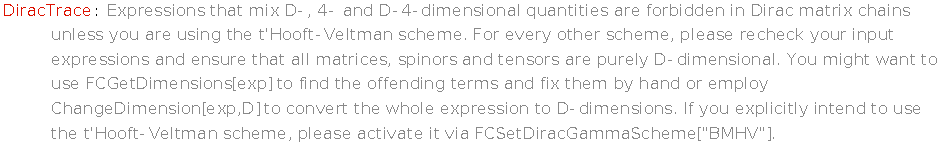
\includegraphics[width=0.6\linewidth]{img/1pt4vjhepgnk6.pdf}
\end{figure}
\FloatBarrier

\begin{dmath*}\breakingcomma
\text{\$Aborted}
\end{dmath*}

\begin{Shaded}
\begin{Highlighting}[]
\NormalTok{FCSetDiracGammaScheme}\OperatorTok{[}\StringTok{"BMHV"}\OperatorTok{]}\NormalTok{;}
\end{Highlighting}
\end{Shaded}

\begin{Shaded}
\begin{Highlighting}[]
\NormalTok{ex }\ExtensionTok{=}\NormalTok{ DiracSimplify}\OperatorTok{[}\NormalTok{DiracTrace}\OperatorTok{[}\NormalTok{(}\SpecialCharTok{{-}}\NormalTok{GSD}\OperatorTok{[}\FunctionTok{q}\OperatorTok{]} \SpecialCharTok{+}\NormalTok{ SMP}\OperatorTok{[}\StringTok{"m\_e"}\OperatorTok{]}\NormalTok{) . GA}\OperatorTok{[}\SpecialCharTok{\textbackslash{}}\OperatorTok{[}\NormalTok{Nu}\OperatorTok{]]}\NormalTok{ . (GS}\OperatorTok{[}\FunctionTok{p}\OperatorTok{]} \SpecialCharTok{{-}}\NormalTok{ GSD}\OperatorTok{[}\FunctionTok{q}\OperatorTok{]} \SpecialCharTok{+}\NormalTok{ SMP}\OperatorTok{[}\StringTok{"m\_e"}\OperatorTok{]}\NormalTok{) . GA}\OperatorTok{[}\SpecialCharTok{\textbackslash{}}\OperatorTok{[}\NormalTok{Mu}\OperatorTok{]]]} \OperatorTok{]}
\end{Highlighting}
\end{Shaded}

\begin{dmath*}\breakingcomma
4 m_e^2 \bar{g}^{\mu \nu }+4 \bar{g}^{\mu \nu } \left(\overline{p}\cdot \overline{q}\right)-4 q^2 \bar{g}^{\mu \nu }-4 \overline{p}^{\nu } \overline{q}^{\mu }-4 \overline{p}^{\mu } \overline{q}^{\nu }+8 \overline{q}^{\mu } \overline{q}^{\nu }
\end{dmath*}

\begin{Shaded}
\begin{Highlighting}[]
\NormalTok{ex }\SpecialCharTok{//}\NormalTok{ FCE }\SpecialCharTok{//} \FunctionTok{StandardForm}

\CommentTok{(*{-}4 FV[p, \textbackslash{}[Nu]] FV[q, \textbackslash{}[Mu]] {-} 4 FV[p, \textbackslash{}[Mu]] FV[q, \textbackslash{}[Nu]] + 8 FV[q, \textbackslash{}[Mu]] FV[q, \textbackslash{}[Nu]] + 4 MT[\textbackslash{}[Mu], \textbackslash{}[Nu]] SMP["m\_e"]\^{}2 + 4 MT[\textbackslash{}[Mu], \textbackslash{}[Nu]] SP[p, q] {-} 4 MT[\textbackslash{}[Mu], \textbackslash{}[Nu]] SPD[q, q]*)}
\end{Highlighting}
\end{Shaded}

\begin{Shaded}
\begin{Highlighting}[]
\NormalTok{FCSetDiracGammaScheme}\OperatorTok{[}\StringTok{"NDR"}\OperatorTok{]}\NormalTok{;}
\end{Highlighting}
\end{Shaded}

Notice that in this case the result contains \(4\)- and
\(D\)-dimensional tensors.

Traces involving \(\gamma^5\) in the BMHV scheme are evaluated using
West's formula. It is possible to turn it off by setting the option
\texttt{West} to \texttt{False}, but then the evaluation will require
much more time.

\begin{Shaded}
\begin{Highlighting}[]
\NormalTok{FCSetDiracGammaScheme}\OperatorTok{[}\StringTok{"BMHV"}\OperatorTok{]}\NormalTok{; }
 
\FunctionTok{AbsoluteTiming}\OperatorTok{[}\NormalTok{r1 }\ExtensionTok{=}\NormalTok{ DiracSimplify}\OperatorTok{[}\NormalTok{DiracTrace}\OperatorTok{[}\NormalTok{GAD}\OperatorTok{[}\SpecialCharTok{\textbackslash{}}\OperatorTok{[}\NormalTok{Mu}\OperatorTok{],} \SpecialCharTok{\textbackslash{}}\OperatorTok{[}\NormalTok{Nu}\OperatorTok{],} \SpecialCharTok{\textbackslash{}}\OperatorTok{[}\NormalTok{Rho}\OperatorTok{]]}\NormalTok{ . GA}\OperatorTok{[}\DecValTok{5}\OperatorTok{]}\NormalTok{ . GAD}\OperatorTok{[}\SpecialCharTok{\textbackslash{}}\OperatorTok{[}\NormalTok{Sigma}\OperatorTok{],} \SpecialCharTok{\textbackslash{}}\OperatorTok{[}\NormalTok{Delta}\OperatorTok{],} \SpecialCharTok{\textbackslash{}}\OperatorTok{[}\NormalTok{Tau}\OperatorTok{]]}\NormalTok{ . GA}\OperatorTok{[}\DecValTok{7}\OperatorTok{]]]}\NormalTok{;}\OperatorTok{]}
\end{Highlighting}
\end{Shaded}

\begin{dmath*}\breakingcomma
\{0.225294,\text{Null}\}
\end{dmath*}

\begin{Shaded}
\begin{Highlighting}[]
\FunctionTok{AbsoluteTiming}\OperatorTok{[}\NormalTok{r2 }\ExtensionTok{=}\NormalTok{ DiracSimplify}\OperatorTok{[}\NormalTok{DiracTrace}\OperatorTok{[}\NormalTok{GAD}\OperatorTok{[}\SpecialCharTok{\textbackslash{}}\OperatorTok{[}\NormalTok{Mu}\OperatorTok{],} \SpecialCharTok{\textbackslash{}}\OperatorTok{[}\NormalTok{Nu}\OperatorTok{],} \SpecialCharTok{\textbackslash{}}\OperatorTok{[}\NormalTok{Rho}\OperatorTok{]]}\NormalTok{ . GA}\OperatorTok{[}\DecValTok{5}\OperatorTok{]}\NormalTok{ . GAD}\OperatorTok{[}\SpecialCharTok{\textbackslash{}}\OperatorTok{[}\NormalTok{Sigma}\OperatorTok{],} \SpecialCharTok{\textbackslash{}}\OperatorTok{[}\NormalTok{Delta}\OperatorTok{],} \SpecialCharTok{\textbackslash{}}\OperatorTok{[}\NormalTok{Tau}\OperatorTok{]]}\NormalTok{ . GA}\OperatorTok{[}\DecValTok{7}\OperatorTok{],} 
\NormalTok{      West }\OtherTok{{-}\textgreater{}} \ConstantTok{False}\OperatorTok{]]}\NormalTok{;}\OperatorTok{]}
\end{Highlighting}
\end{Shaded}

\begin{dmath*}\breakingcomma
\{1.82085,\text{Null}\}
\end{dmath*}

\begin{Shaded}
\begin{Highlighting}[]
\NormalTok{r1 }\ExtensionTok{===}\NormalTok{ r2}
\end{Highlighting}
\end{Shaded}

\begin{dmath*}\breakingcomma
\text{True}
\end{dmath*}

\begin{Shaded}
\begin{Highlighting}[]
\NormalTok{FCSetDiracGammaScheme}\OperatorTok{[}\StringTok{"NDR"}\OperatorTok{]}\NormalTok{; }
 
\FunctionTok{ClearAll}\OperatorTok{[}\NormalTok{r1}\OperatorTok{,}\NormalTok{ r2}\OperatorTok{]}
\end{Highlighting}
\end{Shaded}

If you know that traces with one \(\gamma^5\) do not contribute to your
final result, use the new NDR-Discard scheme to put them to zero

\begin{Shaded}
\begin{Highlighting}[]
\NormalTok{FCSetDiracGammaScheme}\OperatorTok{[}\StringTok{"NDR{-}Discard"}\OperatorTok{]}\NormalTok{; }
 
\NormalTok{DiracSimplify}\OperatorTok{[}\NormalTok{DiracTrace}\OperatorTok{[}\NormalTok{GAD}\OperatorTok{[}\SpecialCharTok{\textbackslash{}}\OperatorTok{[}\NormalTok{Mu}\OperatorTok{],} \SpecialCharTok{\textbackslash{}}\OperatorTok{[}\NormalTok{Nu}\OperatorTok{],} \SpecialCharTok{\textbackslash{}}\OperatorTok{[}\NormalTok{Rho}\OperatorTok{]]}\NormalTok{ . GA}\OperatorTok{[}\DecValTok{5}\OperatorTok{]}\NormalTok{ . GAD}\OperatorTok{[}\SpecialCharTok{\textbackslash{}}\OperatorTok{[}\NormalTok{Sigma}\OperatorTok{],} \SpecialCharTok{\textbackslash{}}\OperatorTok{[}\NormalTok{Delta}\OperatorTok{],} \SpecialCharTok{\textbackslash{}}\OperatorTok{[}\NormalTok{Tau}\OperatorTok{]]}\NormalTok{ . GA}\OperatorTok{[}\DecValTok{7}\OperatorTok{]]]}
\end{Highlighting}
\end{Shaded}

\begin{dmath*}\breakingcomma
2 g^{\delta \tau } g^{\mu \sigma } g^{\nu \rho }+2 g^{\delta \sigma } g^{\mu \tau } g^{\nu \rho }-2 g^{\delta \mu } g^{\nu \rho } g^{\sigma \tau }-2 g^{\delta \tau } g^{\mu \rho } g^{\nu \sigma }-2 g^{\delta \rho } g^{\mu \tau } g^{\nu \sigma }-2 g^{\delta \sigma } g^{\mu \rho } g^{\nu \tau }+2 g^{\delta \rho } g^{\mu \sigma } g^{\nu \tau }+2 g^{\delta \tau } g^{\mu \nu } g^{\rho \sigma }+2 g^{\delta \nu } g^{\mu \tau } g^{\rho \sigma }-2 g^{\delta \mu } g^{\nu \tau } g^{\rho \sigma }+2 g^{\delta \sigma } g^{\mu \nu } g^{\rho \tau }-2 g^{\delta \nu } g^{\mu \sigma } g^{\rho \tau }+2 g^{\delta \mu } g^{\nu \sigma } g^{\rho \tau }-2 g^{\delta \rho } g^{\mu \nu } g^{\sigma \tau }+2 g^{\delta \nu } g^{\mu \rho } g^{\sigma \tau }
\end{dmath*}

\begin{Shaded}
\begin{Highlighting}[]
\NormalTok{FCSetDiracGammaScheme}\OperatorTok{[}\StringTok{"NDR"}\OperatorTok{]}\NormalTok{;}
\end{Highlighting}
\end{Shaded}

Sorting of the matrices inside \(4\)-dimensional traces helps to avoid
some spurious terms.

\begin{Shaded}
\begin{Highlighting}[]
\NormalTok{DiracTrace}\OperatorTok{[}\NormalTok{GA}\OperatorTok{[}\SpecialCharTok{\textbackslash{}}\OperatorTok{[}\NormalTok{Mu}\OperatorTok{],} \SpecialCharTok{\textbackslash{}}\OperatorTok{[}\NormalTok{Nu}\OperatorTok{],} \DecValTok{5}\OperatorTok{,} \SpecialCharTok{\textbackslash{}}\OperatorTok{[}\NormalTok{Rho}\OperatorTok{],} \SpecialCharTok{\textbackslash{}}\OperatorTok{[}\NormalTok{Sigma}\OperatorTok{],} \SpecialCharTok{\textbackslash{}}\OperatorTok{[}\NormalTok{Tau}\OperatorTok{],} \SpecialCharTok{\textbackslash{}}\OperatorTok{[}\NormalTok{Kappa}\OperatorTok{]],}\NormalTok{ DiracTraceEvaluate }\OtherTok{{-}\textgreater{}} \ConstantTok{True}\OperatorTok{]} \SpecialCharTok{{-}} 
\NormalTok{   DiracTrace}\OperatorTok{[}\NormalTok{GA}\OperatorTok{[}\SpecialCharTok{\textbackslash{}}\OperatorTok{[}\NormalTok{Mu}\OperatorTok{],} \SpecialCharTok{\textbackslash{}}\OperatorTok{[}\NormalTok{Nu}\OperatorTok{],} \SpecialCharTok{\textbackslash{}}\OperatorTok{[}\NormalTok{Rho}\OperatorTok{],} \SpecialCharTok{\textbackslash{}}\OperatorTok{[}\NormalTok{Sigma}\OperatorTok{],} \SpecialCharTok{\textbackslash{}}\OperatorTok{[}\NormalTok{Tau}\OperatorTok{],} \SpecialCharTok{\textbackslash{}}\OperatorTok{[}\NormalTok{Kappa}\OperatorTok{],} \DecValTok{5}\OperatorTok{],}\NormalTok{DiracTraceEvaluate }\OtherTok{{-}\textgreater{}} \ConstantTok{True}\OperatorTok{]} \SpecialCharTok{//} \FunctionTok{Expand}
\end{Highlighting}
\end{Shaded}

\begin{dmath*}\breakingcomma
0
\end{dmath*}

When the sorting is turned off via \texttt{Sort} to \texttt{True}, one
may obtain some spurious terms that vanish by Schouten's identity.

\begin{Shaded}
\begin{Highlighting}[]
\NormalTok{DiracTrace}\OperatorTok{[}\NormalTok{GA}\OperatorTok{[}\SpecialCharTok{\textbackslash{}}\OperatorTok{[}\NormalTok{Mu}\OperatorTok{],} \SpecialCharTok{\textbackslash{}}\OperatorTok{[}\NormalTok{Nu}\OperatorTok{],} \DecValTok{5}\OperatorTok{,} \SpecialCharTok{\textbackslash{}}\OperatorTok{[}\NormalTok{Rho}\OperatorTok{],} \SpecialCharTok{\textbackslash{}}\OperatorTok{[}\NormalTok{Sigma}\OperatorTok{],} \SpecialCharTok{\textbackslash{}}\OperatorTok{[}\NormalTok{Tau}\OperatorTok{],} \SpecialCharTok{\textbackslash{}}\OperatorTok{[}\NormalTok{Kappa}\OperatorTok{]],}\NormalTok{ DiracTraceEvaluate }\OtherTok{{-}\textgreater{}} \ConstantTok{True}\OperatorTok{,} \FunctionTok{Sort} \OtherTok{{-}\textgreater{}} \ConstantTok{False}\OperatorTok{]} \SpecialCharTok{{-}} 
\NormalTok{   DiracTrace}\OperatorTok{[}\NormalTok{GA}\OperatorTok{[}\SpecialCharTok{\textbackslash{}}\OperatorTok{[}\NormalTok{Mu}\OperatorTok{],} \SpecialCharTok{\textbackslash{}}\OperatorTok{[}\NormalTok{Nu}\OperatorTok{],} \SpecialCharTok{\textbackslash{}}\OperatorTok{[}\NormalTok{Rho}\OperatorTok{],} \SpecialCharTok{\textbackslash{}}\OperatorTok{[}\NormalTok{Sigma}\OperatorTok{],} \SpecialCharTok{\textbackslash{}}\OperatorTok{[}\NormalTok{Tau}\OperatorTok{],} \SpecialCharTok{\textbackslash{}}\OperatorTok{[}\NormalTok{Kappa}\OperatorTok{],} \DecValTok{5}\OperatorTok{],}\NormalTok{DiracTraceEvaluate }\OtherTok{{-}\textgreater{}} \ConstantTok{True}\OperatorTok{,} \FunctionTok{Sort} \OtherTok{{-}\textgreater{}} \ConstantTok{False}\OperatorTok{]} \SpecialCharTok{//} \FunctionTok{Expand}
\end{Highlighting}
\end{Shaded}

\begin{dmath*}\breakingcomma
4 i \bar{g}^{\kappa \mu } \bar{\epsilon }^{\nu \rho \sigma \tau }-4 i \bar{g}^{\kappa \nu } \bar{\epsilon }^{\mu \rho \sigma \tau }-4 i \bar{g}^{\kappa \sigma } \bar{\epsilon }^{\mu \nu \rho \tau }+4 i \bar{g}^{\kappa \tau } \bar{\epsilon }^{\mu \nu \rho \sigma }+4 i \bar{g}^{\mu \rho } \bar{\epsilon }^{\kappa \nu \sigma \tau }-4 i \bar{g}^{\nu \rho } \bar{\epsilon }^{\kappa \mu \sigma \tau }+4 i \bar{g}^{\rho \sigma } \bar{\epsilon }^{\kappa \mu \nu \tau }-4 i \bar{g}^{\rho \tau } \bar{\epsilon }^{\kappa \mu \nu \sigma }
\end{dmath*}

The trace of the unit matrix in the Dirac space is fixed to 4, which is
the standard choice in dimensional regularization.

\begin{Shaded}
\begin{Highlighting}[]
\NormalTok{DiracTrace}\OperatorTok{[}\DecValTok{1}\OperatorTok{]} 
 
\NormalTok{DiracSimplify}\OperatorTok{[}\SpecialCharTok{\%}\OperatorTok{]}
\end{Highlighting}
\end{Shaded}

\begin{dmath*}\breakingcomma
\text{tr}(1)
\end{dmath*}

\begin{dmath*}\breakingcomma
4
\end{dmath*}

If, for some reason, this value must be modified, one can do so using
the option \texttt{TraceOfOne}.

\begin{Shaded}
\begin{Highlighting}[]
\NormalTok{DiracTrace}\OperatorTok{[}\DecValTok{1}\OperatorTok{,}\NormalTok{ TraceOfOne }\OtherTok{{-}\textgreater{}} \FunctionTok{D}\OperatorTok{,}\NormalTok{ DiracTraceEvaluate }\OtherTok{{-}\textgreater{}} \ConstantTok{True}\OperatorTok{]}
\end{Highlighting}
\end{Shaded}

\begin{dmath*}\breakingcomma
D
\end{dmath*}

\begin{Shaded}
\begin{Highlighting}[]
\NormalTok{DiracSimplify}\OperatorTok{[}\NormalTok{DiracTrace}\OperatorTok{[}\NormalTok{GAD}\OperatorTok{[}\SpecialCharTok{\textbackslash{}}\OperatorTok{[}\NormalTok{Mu}\OperatorTok{],} \SpecialCharTok{\textbackslash{}}\OperatorTok{[}\NormalTok{Nu}\OperatorTok{]],}\NormalTok{ TraceOfOne }\OtherTok{{-}\textgreater{}} \FunctionTok{D}\OperatorTok{]]}
\end{Highlighting}
\end{Shaded}

\begin{dmath*}\breakingcomma
D g^{\mu \nu }
\end{dmath*}

Since FeynCalc 9.3 it is also possible to compute traces of Dirac
matrices with Cartesian or temporal indices. However, the support of
nonrelativistic calculations is a very new feature, so that things may
not work as smooth as they do for manifestly Lorentz covariant
expressions.

\begin{Shaded}
\begin{Highlighting}[]
\NormalTok{DiracTrace}\OperatorTok{[}\NormalTok{CGAD}\OperatorTok{[}\FunctionTok{i}\OperatorTok{,} \FunctionTok{j}\OperatorTok{,} \FunctionTok{k}\OperatorTok{,} \FunctionTok{l}\OperatorTok{]]} 
 
\NormalTok{DiracSimplify}\OperatorTok{[}\SpecialCharTok{\%}\OperatorTok{]}
\end{Highlighting}
\end{Shaded}

\begin{dmath*}\breakingcomma
\text{tr}\left(\gamma ^i.\gamma ^j.\gamma ^k.\gamma ^l\right)
\end{dmath*}

\begin{dmath*}\breakingcomma
4 \delta ^{il} \delta ^{jk}-4 \delta ^{ik} \delta ^{jl}+4 \delta ^{ij} \delta ^{kl}
\end{dmath*}

\begin{Shaded}
\begin{Highlighting}[]
\NormalTok{DiracTrace}\OperatorTok{[}\NormalTok{CGA}\OperatorTok{[}\FunctionTok{i}\OperatorTok{,} \FunctionTok{j}\OperatorTok{,} \FunctionTok{k}\OperatorTok{,} \FunctionTok{l}\OperatorTok{]}\NormalTok{ . GA}\OperatorTok{[}\DecValTok{6}\OperatorTok{]}\NormalTok{ . CGA}\OperatorTok{[}\FunctionTok{m}\OperatorTok{,} \FunctionTok{n}\OperatorTok{]]} 
 
\NormalTok{DiracSimplify}\OperatorTok{[}\SpecialCharTok{\%}\OperatorTok{]}
\end{Highlighting}
\end{Shaded}

\begin{dmath*}\breakingcomma
\text{tr}\left(\overline{\gamma }^i.\overline{\gamma }^j.\overline{\gamma }^k.\overline{\gamma }^l.\bar{\gamma }^6.\overline{\gamma }^m.\overline{\gamma }^n\right)
\end{dmath*}

\begin{dmath*}\breakingcomma
-2 \bar{\delta }^{in} \bar{\delta }^{jm} \bar{\delta }^{kl}+2 \bar{\delta }^{im} \bar{\delta }^{jn} \bar{\delta }^{kl}-2 \bar{\delta }^{ij} \bar{\delta }^{kl} \bar{\delta }^{mn}+2 \bar{\delta }^{in} \bar{\delta }^{jl} \bar{\delta }^{km}-2 \bar{\delta }^{il} \bar{\delta }^{jn} \bar{\delta }^{km}-2 \bar{\delta }^{im} \bar{\delta }^{jl} \bar{\delta }^{kn}+2 \bar{\delta }^{il} \bar{\delta }^{jm} \bar{\delta }^{kn}-2 \bar{\delta }^{in} \bar{\delta }^{jk} \bar{\delta }^{lm}+2 \bar{\delta }^{ik} \bar{\delta }^{jn} \bar{\delta }^{lm}-2 \bar{\delta }^{ij} \bar{\delta }^{kn} \bar{\delta }^{lm}+2 \bar{\delta }^{im} \bar{\delta }^{jk} \bar{\delta }^{ln}-2 \bar{\delta }^{ik} \bar{\delta }^{jm} \bar{\delta }^{ln}+2 \bar{\delta }^{ij} \bar{\delta }^{km} \bar{\delta }^{ln}-2 \bar{\delta }^{il} \bar{\delta }^{jk} \bar{\delta }^{mn}+2 \bar{\delta }^{ik} \bar{\delta }^{jl} \bar{\delta }^{mn}
\end{dmath*}
\end{document}
